\documentclass[xcolor=table]{beamer}

% \rowcolors{1}{gray!30}{gray!10}

\usetheme{Boadilla}
\usecolortheme{dolphin}
\useoutertheme[subsection=false]{smoothbars}

\setbeamercolor{frametitle}{fg = black, bg = white} 
\setbeamercolor{palette primary}{use=structure,fg=white,bg=structure.fg!60!white}
\setbeamercolor{palette secondary}{use=structure,fg=white,bg=structure.fg!90!white}
\setbeamercolor{palette tertiary}{use=structure,fg=white,bg=structure.fg!120!white}
\setbeamercolor{palette quaternary}{use=structure,fg=black,bg=white} %Top bar

\setbeamertemplate{enumerate subitem}[circle]%
\renewcommand{\insertsubenumlabel}{\alph{enumii}}

\usepackage{amsmath}
\usepackage{xcolor}
\usepackage{booktabs}
\usepackage[utf8]{inputenc}
\usepackage{hyperref}
\usepackage[table]{xcolor}
\definecolor{lightgray}{gray}{0.9}

\hypersetup{
    colorlinks,
    citecolor=blue,
    linkcolor=blue
}

\footnotesize \let\small\footnotesize

\author{Jonathan P. Latner, PhD}
\title{Build a churn model with the following data}
\date{\today}

\beamertemplatenavigationsymbolsempty 
\setbeamerfont{page number in head/foot}{size=\tiny}
\setbeamertemplate{footline}[frame number]
\setbeamertemplate{caption}[numbered]
\setbeamertemplate{section in toc}[sections numbered]

\begin{document}

\section{Introduction}
\frame{\frametitle{ }
\titlepage
\thispagestyle{empty}
}

\frame{\frametitle{Overview} 
\tableofcontents[hideallsubsections]
}

\section{Summary statistics}

\frame{\frametitle{Variables} 
\vskip -10mm
\begin{table}[!h]
    \tiny
    \caption{}
    \rowcolors{2}{gray!50}{gray!10}
    \begin{center}
        \begin{tabular}{rllr}
\toprule
 number &          variable &    type &  count \\
\midrule
      1 &             state &  factor &      1 \\
      2 &           country &  factor &      1 \\
      3 &       churn\_label &  factor &      2 \\
      4 &    senior\_citizen &  factor &      2 \\
      5 &     phone\_service &  factor &      2 \\
      6 &        dependents &  factor &      2 \\
      7 &           partner &  factor &      2 \\
      8 &            gender &  factor &      2 \\
      9 & paperless\_billing &  factor &      2 \\
     10 &  streaming\_movies &  factor &      3 \\
     11 &   online\_security &  factor &      3 \\
     12 &     online\_backup &  factor &      3 \\
     13 &    multiple\_lines &  factor &      3 \\
     14 &  internet\_service &  factor &      3 \\
     15 & device\_protection &  factor &      3 \\
     16 &          contract &  factor &      3 \\
     17 &      streaming\_tv &  factor &      3 \\
     18 &      tech\_support &  factor &      3 \\
     19 &    payment\_method &  factor &      4 \\
     20 &      churn\_reason &  factor &     21 \\
     21 &              city &  factor &   1129 \\
     22 &          lat\_long &  factor &   1652 \\
     23 &        customerid &  factor &   7043 \\
     24 &          zip\_code & numeric &      1 \\
     25 &          latitude & numeric &      1 \\
     26 &         longitude & numeric &      1 \\
     27 &     tenure\_months & numeric &      1 \\
     28 &   monthly\_charges & numeric &      1 \\
     29 &     total\_charges & numeric &      1 \\
\bottomrule
\end{tabular}

        \label{table_variables}
    \end{center}
\end{table}
}

\frame{\frametitle{Missing values}
Who are the missings $total\_charges$?  Customers in their first month  
\begin{figure}
    \caption{}
    \resizebox{\textwidth}{!}{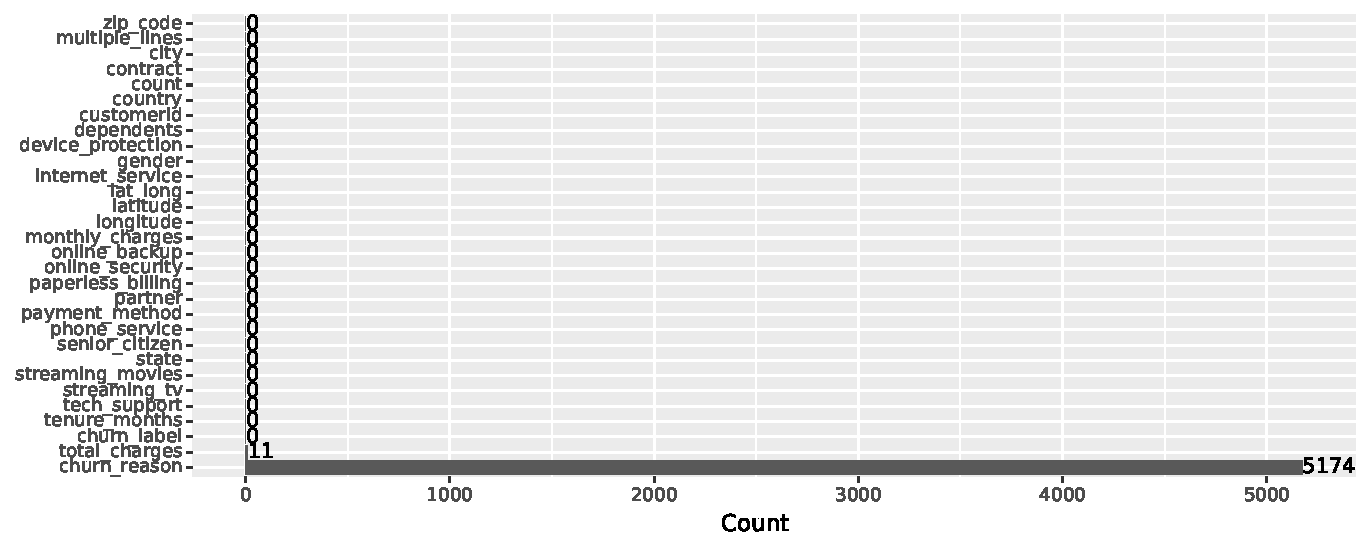
\includegraphics{../graphs/graph_missing.pdf}}
    \label{graph_missing}
\end{figure}
}

\frame{\frametitle{Customer churn}
Need to over sample the training dataset because only 27\% churn (DV)

\begin{figure}
    \caption{}
    \resizebox{\textwidth}{!}{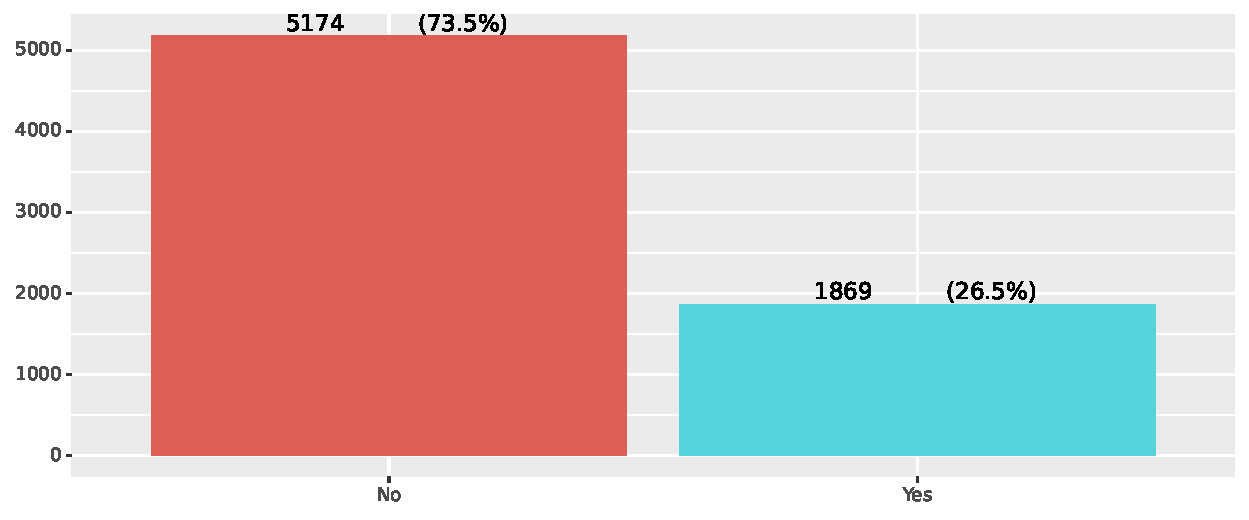
\includegraphics{../graphs/graph_churn.pdf}}
    \label{graph_churn}
\end{figure}
}

\frame{\frametitle{Customer churn by demographics}
Households w/o children, single, and seniors more likely to churn

\begin{figure}
    \caption{}
    \resizebox{\textwidth}{!}{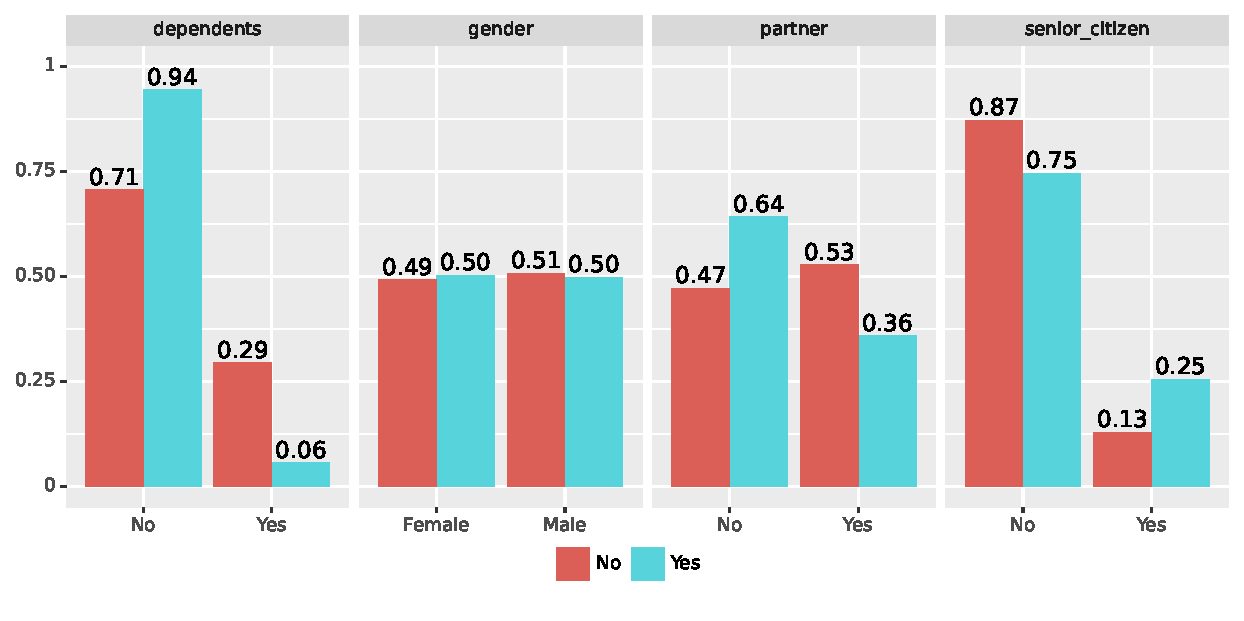
\includegraphics{../graphs/graph_churn_demographics.pdf}}
    \label{graph_churn_demographics}
\end{figure}
}

\frame{\frametitle{Customer churn by services}
Households w/ internet, but w/o online services (except streaming) most likely to churn

\begin{figure}
    \caption{}
    \resizebox{\textwidth}{!}{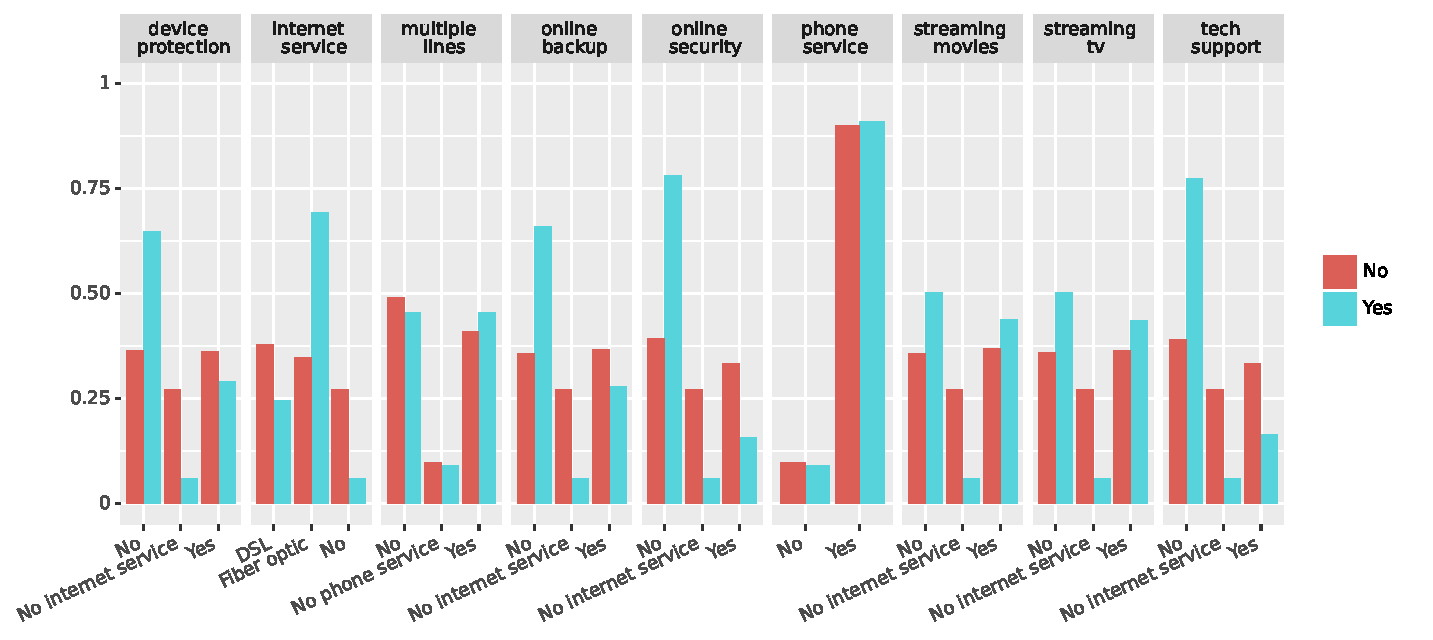
\includegraphics{../graphs/graph_churn_services.pdf}}
    \label{graph_churn_services}
\end{figure}
}

\frame{\frametitle{Customer churn by contract type}
Households w/ monthly contracts, paperless billing (i.e. contact), or electronic checks most likely to churn

\begin{figure}
    \caption{}
    \resizebox{\textwidth}{!}{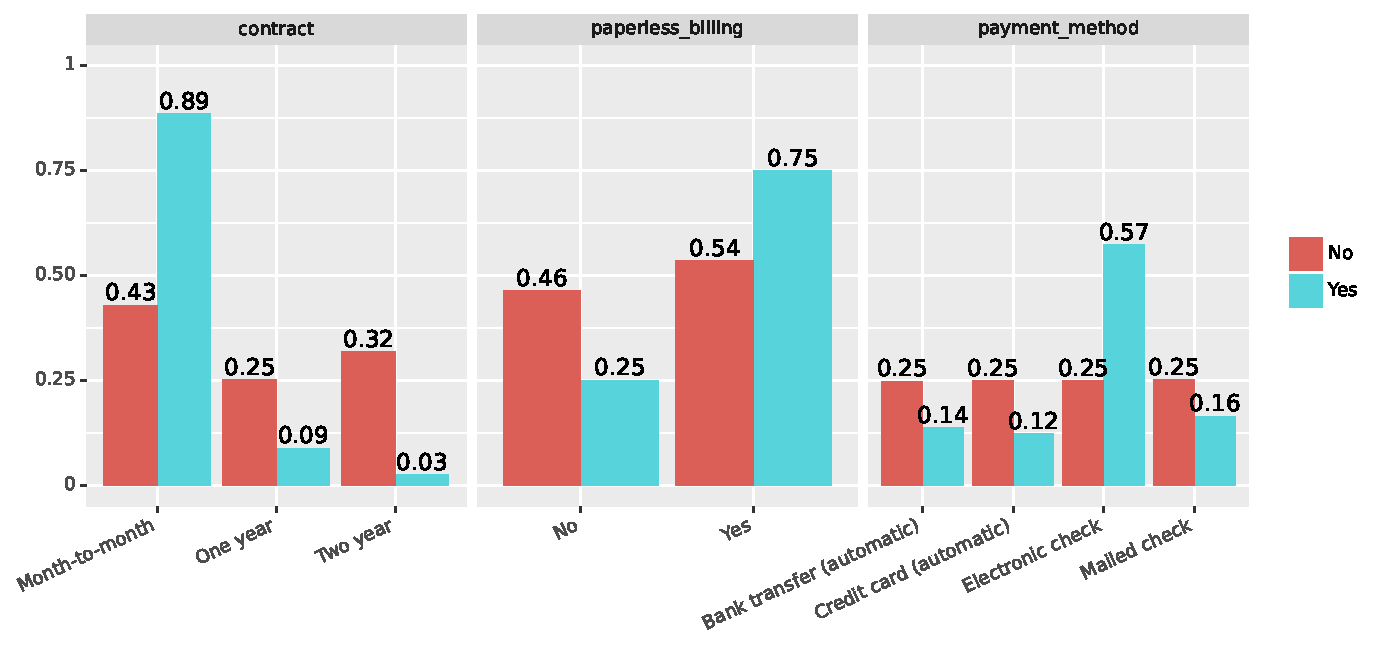
\includegraphics{../graphs/graph_churn_contract_type.pdf}}
    \label{graph_churn_contract_type}
\end{figure}
}

\frame{\frametitle{Customer churn by contract charges}
Higher monthly charges, lower tenure months, and higher total charges more likely to churn.  

Tenure explains inverse relationship between total charges and churn.

\begin{figure}
    \caption{}
    \resizebox{\textwidth}{!}{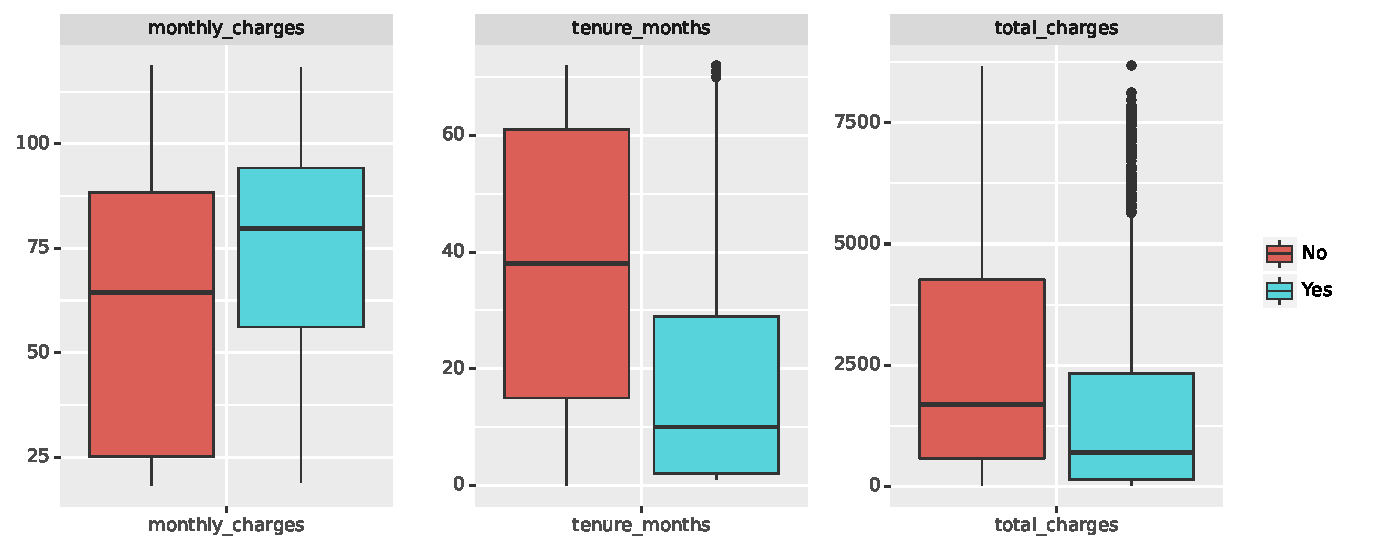
\includegraphics{../graphs/graph_churn_contract_charges.pdf}}
    \label{graph_churn_contract_charges}
\end{figure}
}

\frame{\frametitle{Multivariate correlation}
\begin{small}
High correlation between $tenure\_months$, $monthly\_charges$, $total\_charges$

High correlation between $monthly\_charges$,  $internet\_service\_no$, $internet\_service\_fiber\_optic$
\end{small}

\vspace{-5 mm}
\begin{figure}
    \caption{}
    \resizebox{\textwidth}{!}{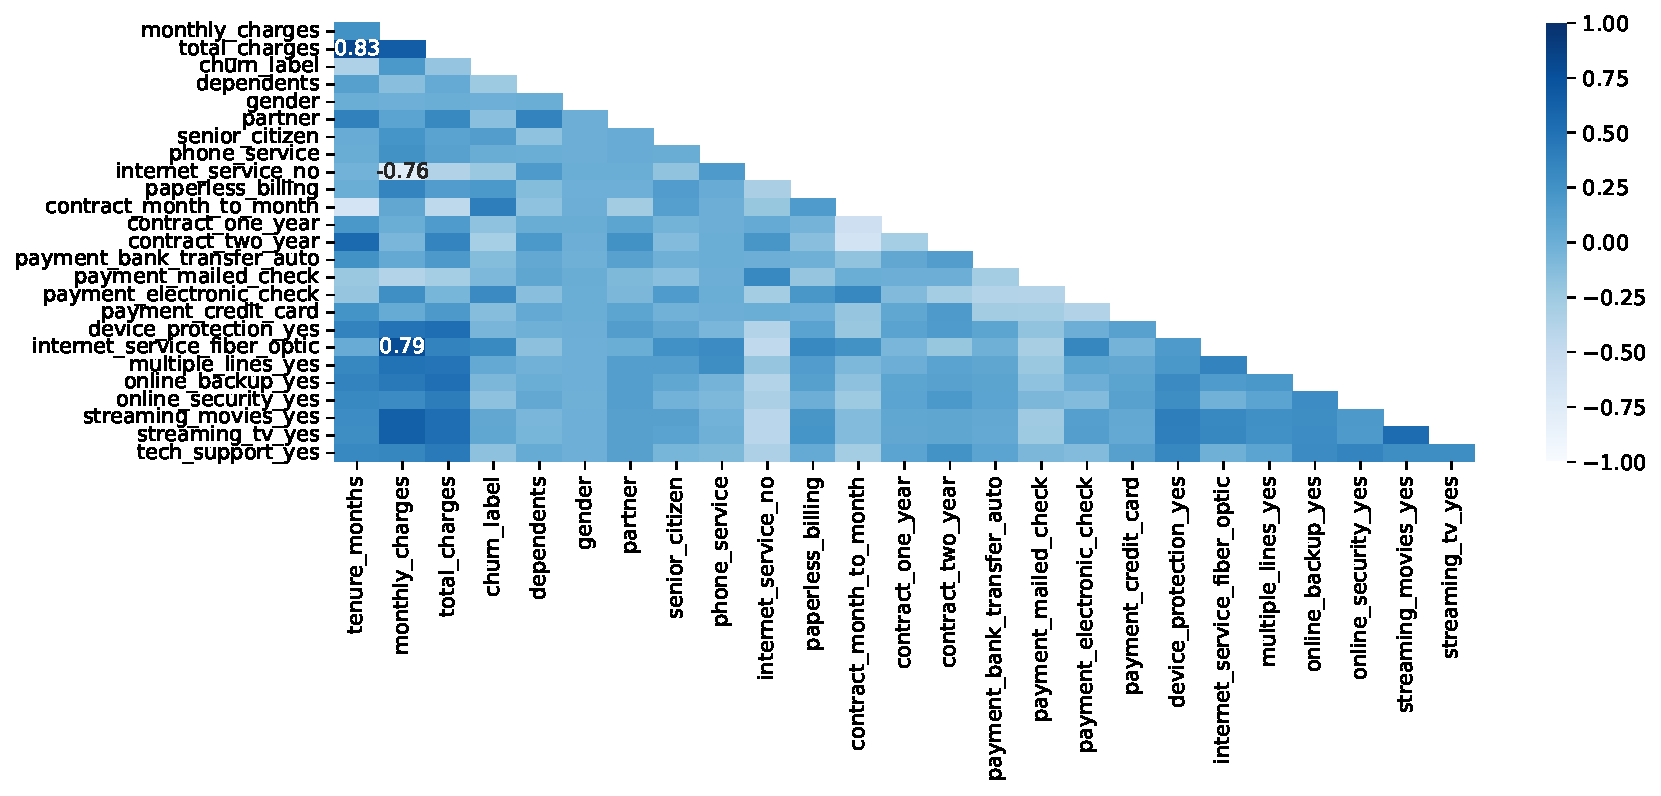
\includegraphics{../graphs/multivaritate_corr_finaldf.pdf}}
    \label{graph_multivaritate_corr_finaldf}
\end{figure}
}

\section{GLM}
\frame{\frametitle{Variance inflation factors (VIF)} 

\begin{small}
    Drop $monthly\_charges$, $total\_charges$, $phone\_service$?

    Keep $tenure\_months$?
\end{small}

\vspace{-5 mm}
\begin{table}[!h]
    \tiny
    \caption{}
    \rowcolors{2}{gray!50}{gray!10}
    \begin{center}
        \begin{tabular}{lrrrr}
\toprule
                    Features &  VIF\_1 &  VIF\_2 &  VIF\_3 &  VIF\_4 \\
\midrule
             monthly\_charges &  13.70 &    NaN &    NaN &    NaN \\
               total\_charges &  10.88 &   9.63 &    NaN &    NaN \\
               phone\_service &  10.51 &  10.33 &  10.33 &    NaN \\
internet\_service\_fiber\_optic &   9.34 &   4.99 &   4.45 &   3.47 \\
               tenure\_months &   9.28 &   9.27 &   2.51 &   2.07 \\
         internet\_service\_no &   5.44 &   2.82 &   2.66 &   1.92 \\
    payment\_electronic\_check &   3.50 &   3.20 &   2.99 &   2.90 \\
           paperless\_billing &   3.30 &   3.11 &   3.08 &   2.99 \\
            streaming\_tv\_yes &   3.07 &   2.74 &   2.67 &   2.67 \\
        streaming\_movies\_yes &   3.06 &   2.74 &   2.67 &   2.67 \\
           contract\_two\_year &   3.05 &   2.98 &   2.86 &   2.79 \\
          multiple\_lines\_yes &   2.60 &   2.48 &   2.44 &   2.27 \\
                     partner &   2.28 &   2.24 &   2.23 &   2.21 \\
       device\_protection\_yes &   2.08 &   2.07 &   2.03 &   2.02 \\
  payment\_bank\_transfer\_auto &   2.05 &   1.91 &   1.83 &   1.76 \\
         payment\_credit\_card &   1.99 &   1.88 &   1.82 &   1.75 \\
            tech\_support\_yes &   1.97 &   1.97 &   1.92 &   1.88 \\
                      gender &   1.97 &   1.87 &   1.87 &   1.82 \\
           contract\_one\_year &   1.92 &   1.87 &   1.85 &   1.81 \\
           online\_backup\_yes &   1.89 &   1.89 &   1.84 &   1.82 \\
         online\_security\_yes &   1.76 &   1.76 &   1.74 &   1.67 \\
                  dependents &   1.48 &   1.48 &   1.47 &   1.47 \\
              senior\_citizen &   1.33 &   1.32 &   1.32 &   1.32 \\
\bottomrule
\end{tabular}

        \label{table_vif_3}
    \end{center}
\end{table}
}

\frame{\frametitle{Accuracy} 

\begin{itemize}
    \item No real gain/loss in accuracy with different GLM model specifications 
    \item Choose model 4: Drop $monthly\_charges$, $total\_charges$,  $phone\_service$
        \begin{itemize}
            \item total charges are a result of monthly charges and tenure 
            \item Monthly charges are a result of services.
            \item 90\% of customers have phone service \& no difference in churn
        \end{itemize}
\end{itemize}

\begin{table}[!h]
    % \tiny
    \caption{}
    \rowcolors{2}{gray!50}{gray!10}
    \begin{center}
        \begin{tabular}{lrrrr}
\toprule
measure &  model\_1 &  model\_2 &  model\_3 &  model\_4 \\
\midrule
     TN &    0.390 &    0.377 &    0.385 &    0.385 \\
     FP &    0.110 &    0.123 &    0.115 &    0.115 \\
     FN &    0.066 &    0.067 &    0.081 &    0.082 \\
     TP &    0.434 &    0.433 &    0.419 &    0.418 \\
    ACC &    0.824 &    0.810 &    0.804 &    0.803 \\
\bottomrule
\end{tabular}

        \label{table_cm_3}
    \end{center}
\end{table}
}

\section{Compare}
\frame{\frametitle{Compare training models on test data}

Random forest (RF) is most accurate, but GLM higher true positive (TP)

Choose GLM model

\begin{table}[!h]
    % \tiny
    \caption{}
    \rowcolors{2}{gray!50}{gray!10}
    \begin{center}
        \begin{tabular}{lrrrrr}
\toprule
measure &   GLM &   KNN &    NB &    DT &    RF \\
\midrule
     TN & 0.557 & 0.490 & 0.563 & 0.574 & 0.592 \\
     FP & 0.174 & 0.242 & 0.169 & 0.157 & 0.140 \\
     FN & 0.072 & 0.045 & 0.073 & 0.111 & 0.100 \\
     TP & 0.196 & 0.224 & 0.196 & 0.157 & 0.168 \\
    ACC & 0.754 & 0.714 & 0.759 & 0.731 & 0.760 \\
\bottomrule
\end{tabular}

        \label{table_cm_compare}
    \end{center}
\end{table}
}

\frame{\frametitle{Examine preferred GLM model }

\begin{figure}
    \caption{Odds ratios}
    \resizebox{\textwidth}{!}{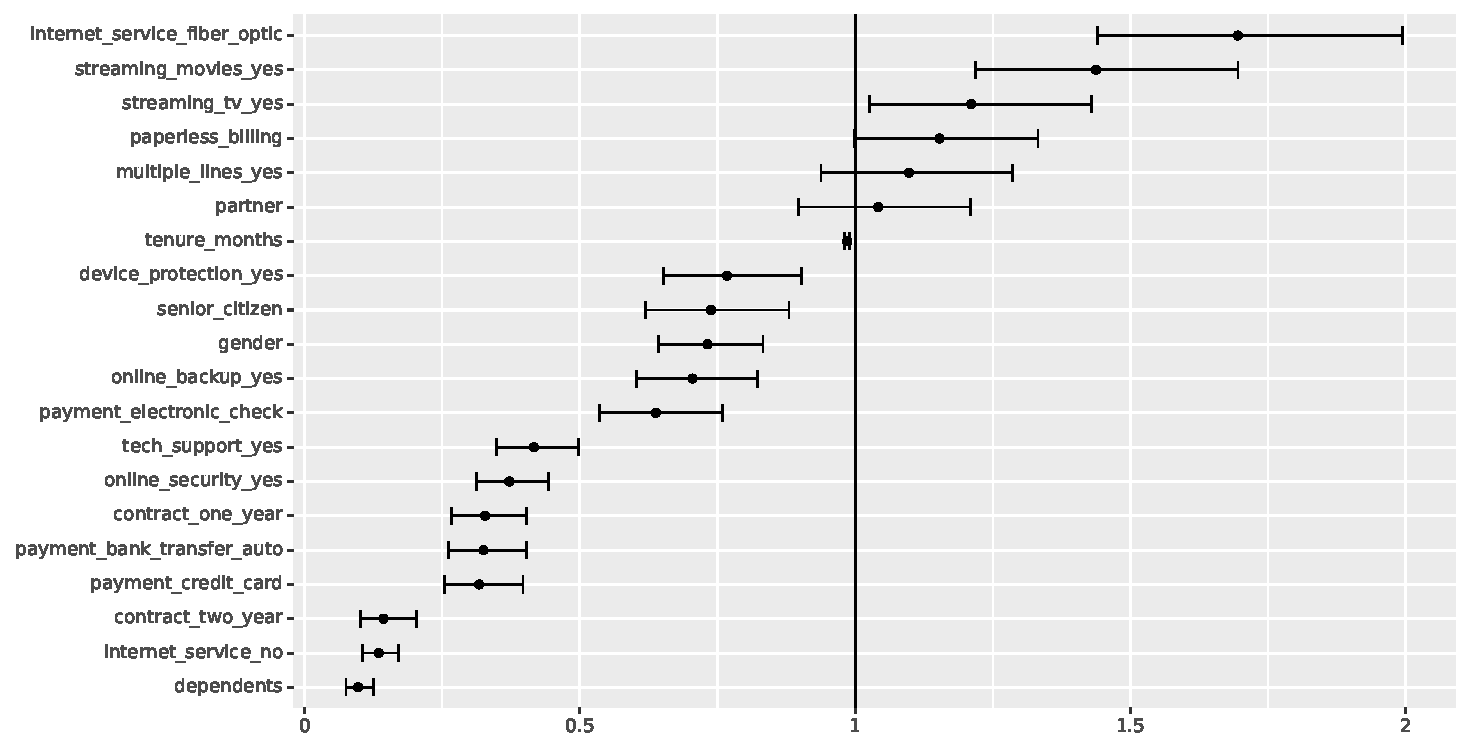
\includegraphics{../graphs/graph_glm.pdf}}
    \label{graph_glm}
\end{figure}
}

\section{Survival}
\frame{\frametitle{KM curve}

After 72 months (the max tenure in our data), the company can retain $\approx$ 60\% of its customers.

\begin{figure}
    \caption{}
    \resizebox{\textwidth}{!}{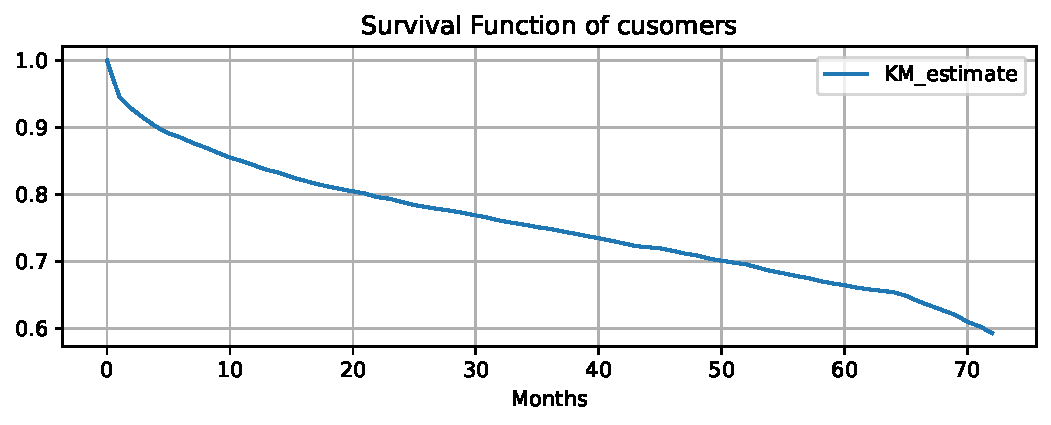
\includegraphics{../graphs/km_curve.pdf}}
    \label{graph_km_curve}
\end{figure}
}

\frame{\frametitle{KM curve by internet service}

After 72 months, the company retains 42\% Fiber optic, 72\% DSL, and 90\% without internet.  Is internet not good or too expensive?

\begin{figure}
    \caption{}
    \resizebox{\textwidth}{!}{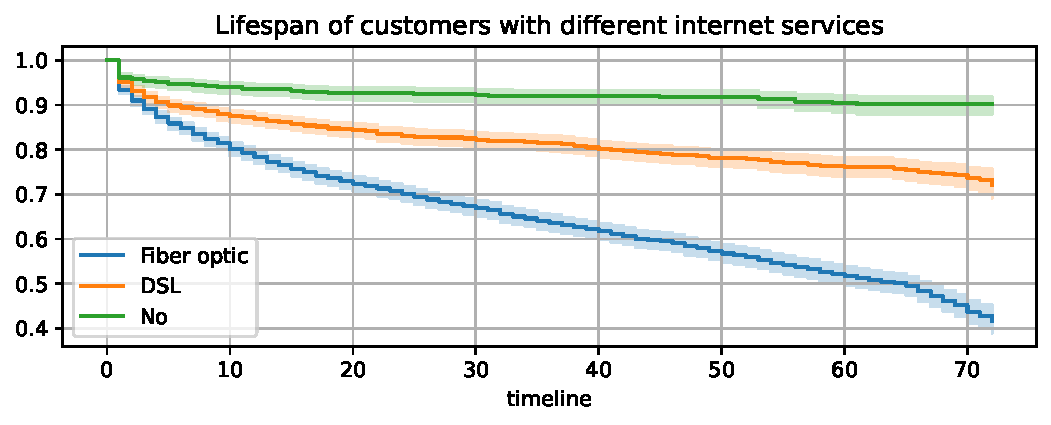
\includegraphics{../graphs/km_curve_internet.pdf}}
    \label{graph_km_curve_internet}
\end{figure}
}
\frame{\frametitle{KM curve by contract type}

After 72 months, the company retains 13\% month-to-month, 57\% one year contract, and 94\% two year contract

\begin{figure}
    \caption{}
    \resizebox{\textwidth}{!}{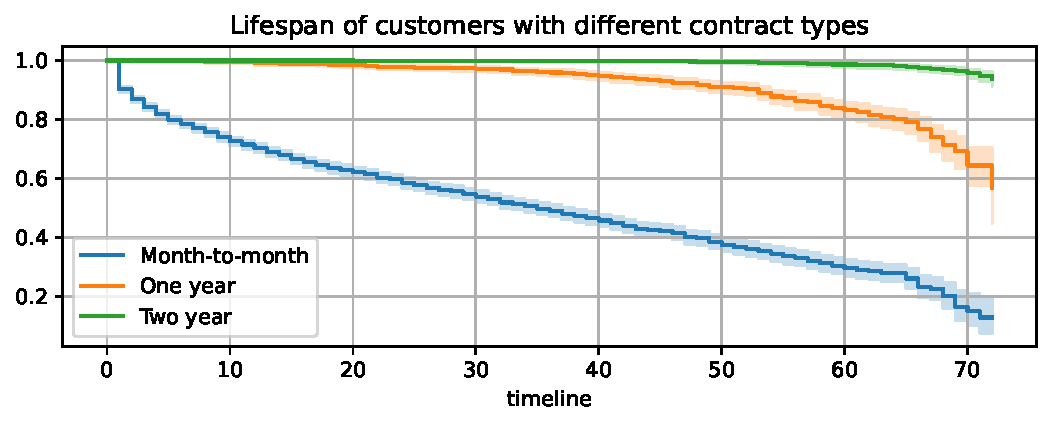
\includegraphics{../graphs/km_curve_contract.pdf}}
    \label{graph_km_curve_contract}
\end{figure}
}

\frame{\frametitle{KM curve by payment type}

After 72 months, the company retains 29\% electronic check compared to $\approx$ 75\% other forms of payment

\begin{figure}
    \caption{}
    \resizebox{\textwidth}{!}{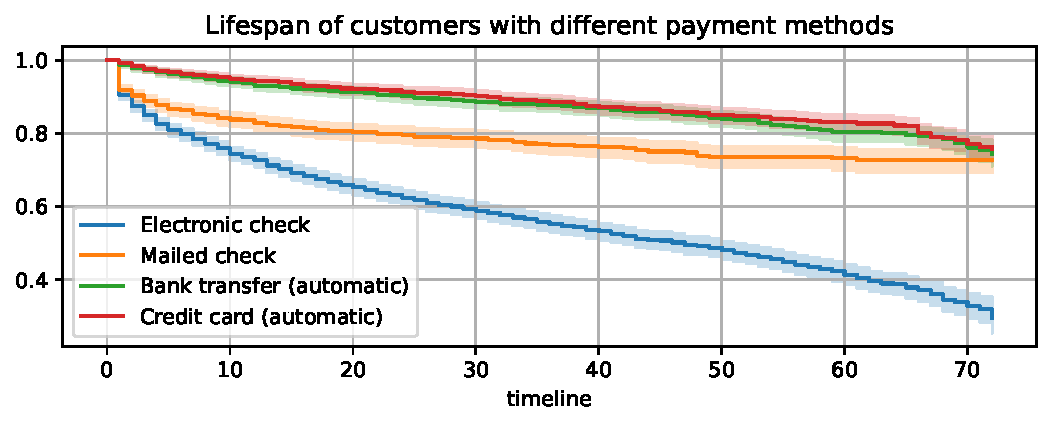
\includegraphics{../graphs/km_curve_payment.pdf}}
    \label{graph_km_curve_payment}
\end{figure}
}



\frame{\frametitle{Cox proportional hazard (CPH) model}

\begin{figure}
    \caption{}
    \resizebox{\textwidth}{!}{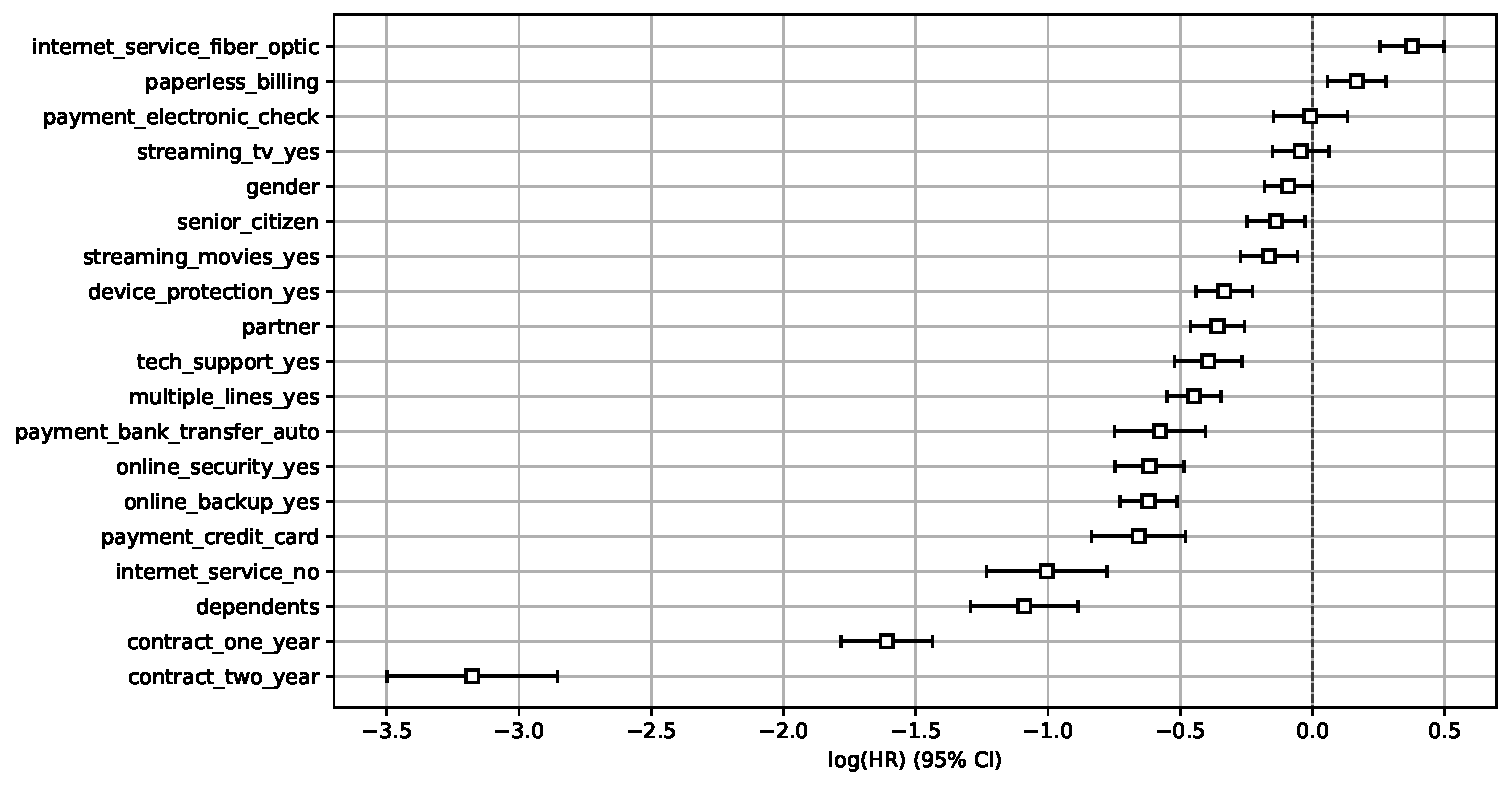
\includegraphics{../graphs/cph_coef.pdf}}
    \label{graph_cph_coef}
\end{figure}
}

\section{Segmentation}
\frame{\frametitle{Customers by all available services}
\begin{figure}
    \caption{}
    \vspace{-5 mm}
    \resizebox{\textwidth}{!}{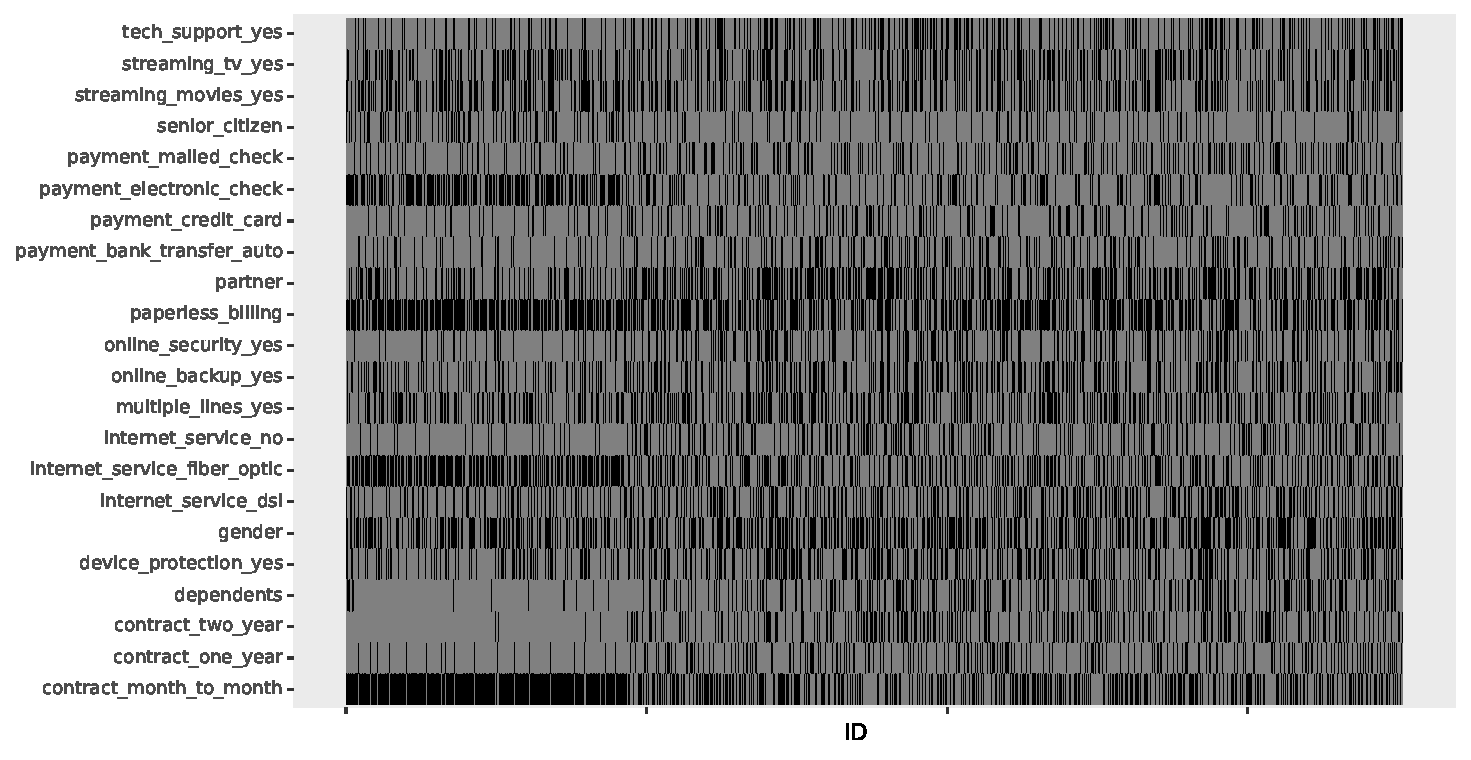
\includegraphics{../graphs/graph_customers.pdf}}
    \label{graph_customers}
\end{figure}
}

\frame{\frametitle{Customers by segment}
Divide into distinct groups using k-means clustering

\begin{figure}
    \caption{}
    \vspace{-5 mm}
    \resizebox{\textwidth}{!}{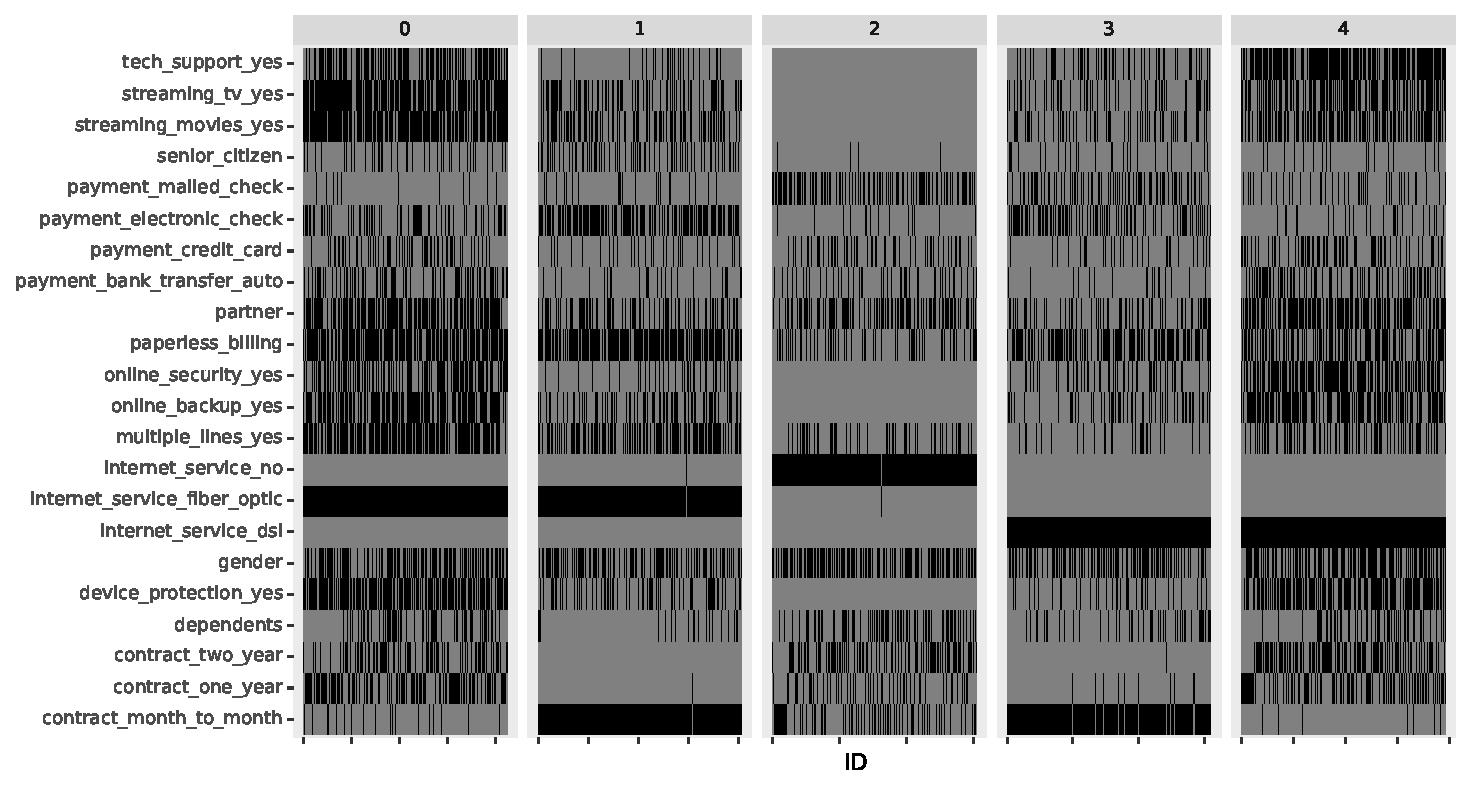
\includegraphics{../graphs/graph_customers_cluster.pdf}}
    \label{graph_customers_cluster}
\end{figure}
}

\frame{\frametitle{Customer segment group by percent}

\begin{figure}
    \caption{}
    \resizebox{\textwidth}{!}{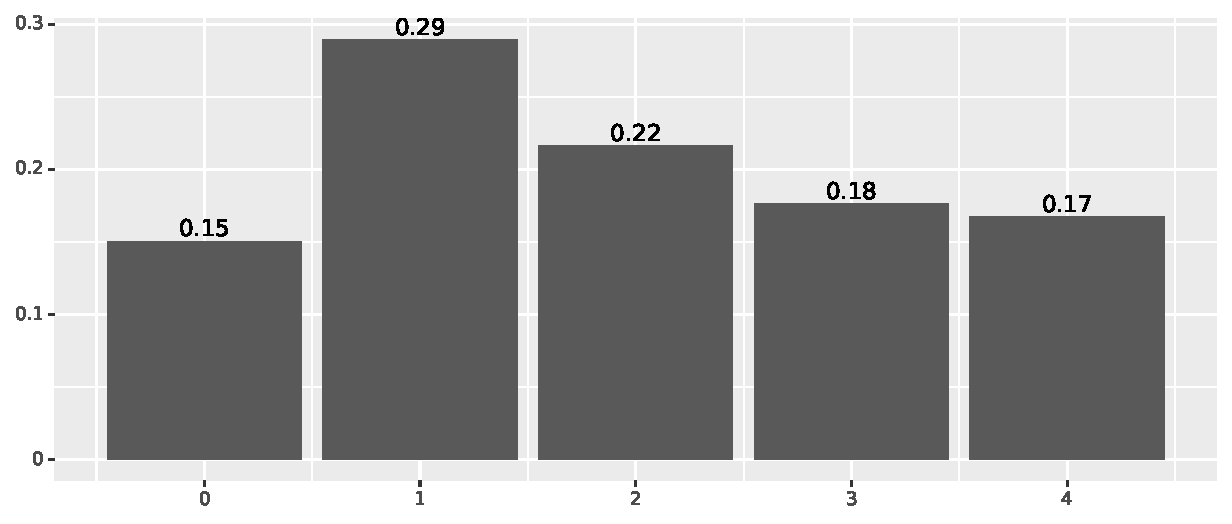
\includegraphics{../graphs/graph_segment.pdf}}
    \label{graph_segment}
\end{figure}
}

\frame{\frametitle{Customer churn by segment group}

2 Segments are most likely to churn

\begin{figure}
    \caption{}
    \resizebox{\textwidth}{!}{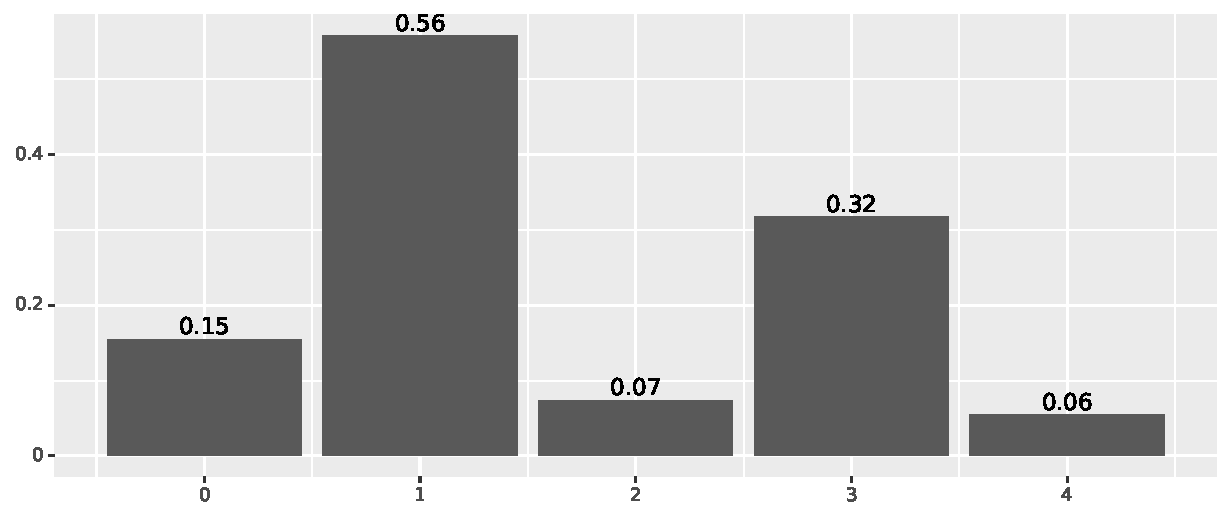
\includegraphics{../graphs/graph_segment_churn.pdf}}
    \label{graph_segment_churn}
\end{figure}
}

\frame{\frametitle{Customer segmentation analysis} 

\begin{itemize}
    \item Key point: month-to-month customers are most likely to churn
    \item 4 distinct groups
    \item 2 groups with month-to-month most likely to churn
    \begin{itemize}
        \item 1 group has fiber optic
        \item 1 group has no internet
    \end{itemize}
    \item 2 groups without month-to-month less likely to churn
    \begin{itemize}
        \item 1 group has fiber optic
        \item 1 group has no internet
    \end{itemize}
\end{itemize}
}


\section{Conclusion}
\frame[c]{\frametitle{}
\centering
Thank you
}



\end{document}


